\section{Design}
\subsection{Requirements and Tasks}
Design a reactor small enough to fit through a door.
The magnetic (vacuum) field of the reactor should be "small and fat", in this case meaning a large volume with a small aspect ratio.
Additionally, a minimal possible number of unique coil types should be achieved for ease of manufacturing.
The design must be scalable in a way such that the minimum inter-coil distance for the model does not subceed $15~\unit{mm}$.



\subsection{Outcome}
After searching the \href{https://quasr.flatironinstitute.org/}{QUASR} data base it was decided that \cite{QUASR}, a design with 3 distinct coil types and an aspect ratio of about 4 shall serve as the base, with the possibility of further optimizations being performed on it using \href{https://github.com/hiddenSymmetries/simsopt}{SIMSOPT}, \href{https://github.com/PrincetonUniversity/STELLOPT}{STELLOPT}, and \href{https://github.com/itpplasma/SIMPLE}{SIMPLE} (for alpha particle tracing).
\autoref{tab:conffrac} shows the calculated alpha particle losses for certain magnetic flux surfaces, both for the small model and a scale-up.

\begin{table}[H]
    \caption{Confined alpha particle fraction on certain magnetic flux surfaces sbeg for one specific run of \href{https://github.com/itpplasma/SIMPLE}{SIMPLE}, for both the small model as well as a model scaled to the plasma volume of \href{https://www.ipp.mpg.de/wendelstein7x}{Wendelstein 7-X.}\\
    $sbeg$... Flux surface on which the particle tracing starts\\  
    $c_f$... Confined fraction of the plasma remaining after 10 ms\\
    $c_{f,\text{scaled}}$...confined fraction of a scaled up system $B_{fac}=5$, $R_{fac}=11.13$)}
    \centering
    \begin{tabular}{c c c}
        sbeg & $c_f$ & $c_{f,\text{scaled}}$ \\
        \hline
        0.1 & 0.63 & 0.85 \\
        0.2 & 0.56 & 0.77 \\
        0.3 & 0.54 & 0.77 \\
        0.4 & 0.49 & 0.76 \\
        0.5 & 0.46 & 0.72 \\
        0.6 & 0.41 & 0.71 \\
        0.7 & 0.42 & 0.75 \\
        0.8 & 0.43 & 0.71 \\
        0.9 & 0.35 & 0.69 \\
    \end{tabular}
    \label{tab:conffrac}
\end{table}
An exemplary plot of Poincaré slices for the (not further optimized) vacuum field in case of a shifted coil can be seen in \autoref{fig:poincare_shifted_coils}.

\begin{figure}[H]
\centering
\captionsetup[subfigure]{justification=centering}
\begin{subfigure}{1.0\textwidth}
\centering
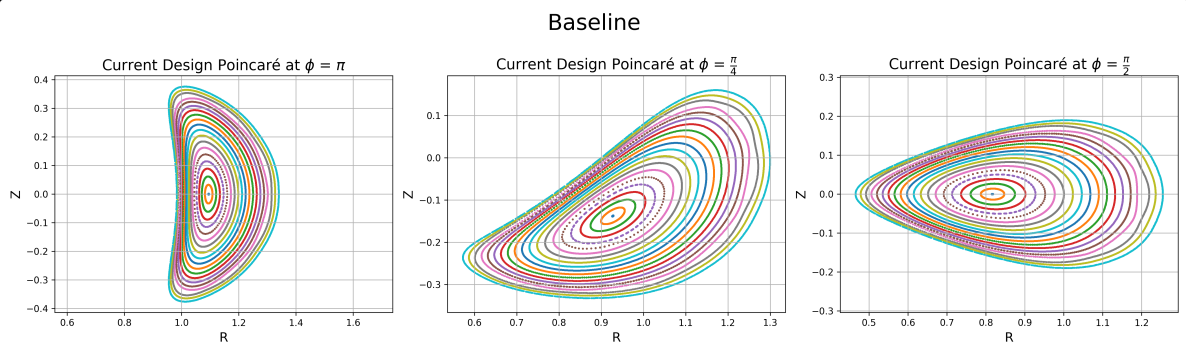
\includegraphics[width=1.0\linewidth]{Images/03_Design/good.png}
\caption{Baseline/unshifted coils}
\label{fig:unshifted}
\end{subfigure}
\end{figure}

\begin{figure}[H]
\ContinuedFloat
\captionsetup[subfigure]{justification=centering}
\begin{subfigure}{1.0\textwidth}
\centering
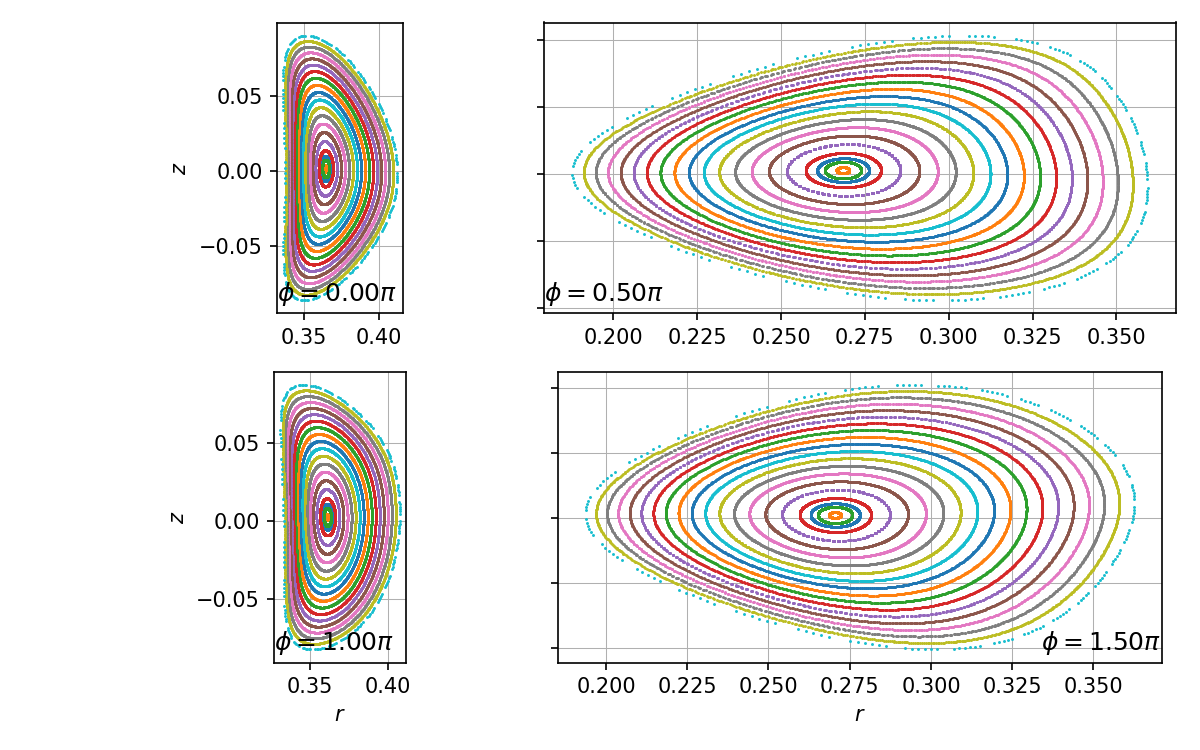
\includegraphics[scale=0.7]{Images/03_Design/1cm.png}
\caption{One coil shifted by 1 cm.}
\label{fig:1cm_shifted}
\end{subfigure}
\end{figure}

\begin{figure}[H]
\captionsetup[subfigure]{justification=centering}
\ContinuedFloat
\begin{subfigure}{1.0\textwidth}
\centering
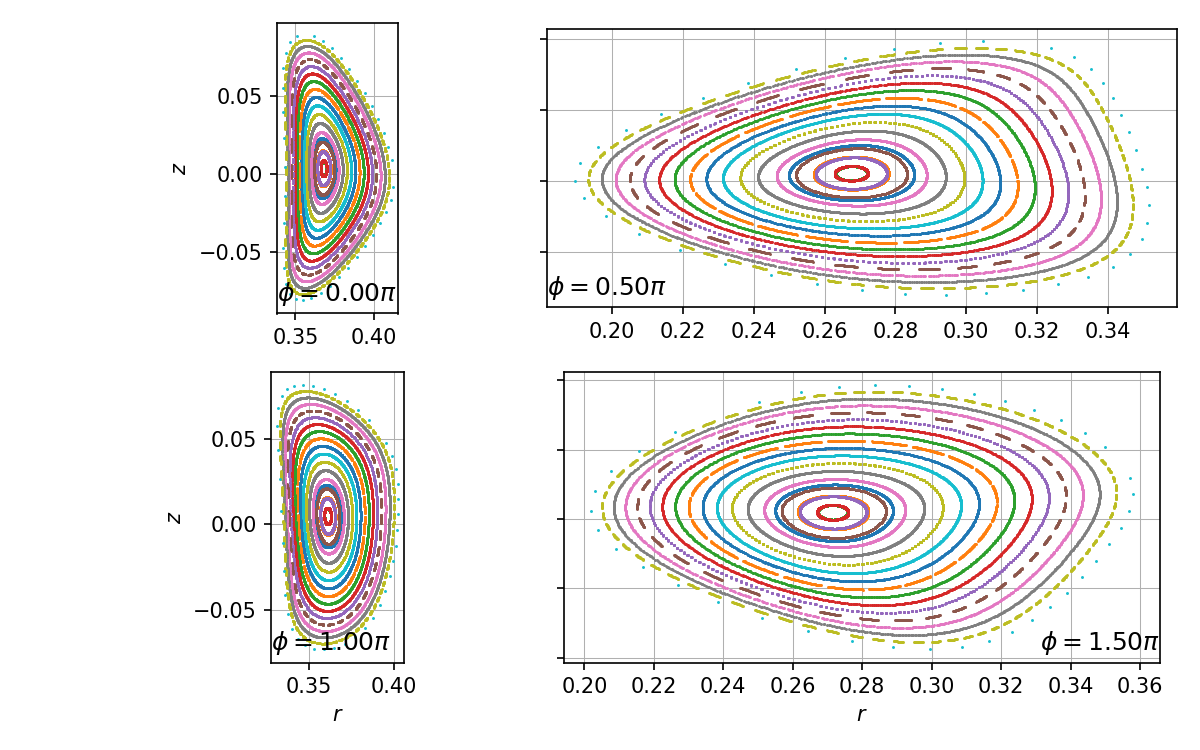
\includegraphics[scale=0.7]{Images/03_Design/2cm.png}
\caption{One coil shifted by 2 cm.}
\label{fig:2cm_shifted}
\end{subfigure}
\end{figure}

\begin{figure}[H]
\captionsetup[subfigure]{justification=centering}
\ContinuedFloat
\begin{subfigure}{1.0\textwidth}
\centering
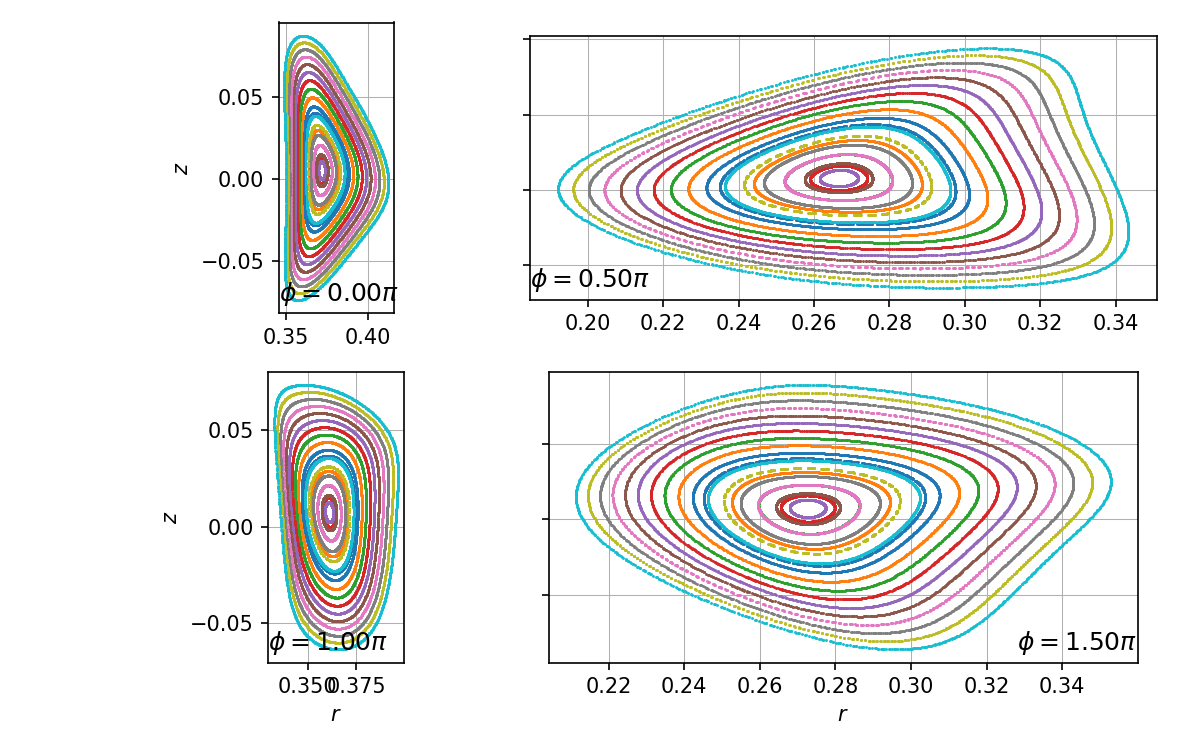
\includegraphics[scale=0.7]{Images/03_Design/3cm.png}
\caption{One coil shifted by 3 cm.}
\label{fig:3cm_shifted}
\end{subfigure}

\caption{Poincare plots for the fields of a) unshifted coils, b), c), d) one coil shifted.}
\label{fig:poincare_shifted_coils}
\end{figure}

Further results on the influence of manufacturing and positioning errors of the coils can be found at \href{https://github.com/itpplasma/reactor24}{this Github repository} \cite{design_repo}.

\subsection{Outlook}
Further optimization could yield an even lower aspect ratio.
One must take note of the coil shape however, as the inter-coil distance of the design refers to infinitesimally thin coils, meaning one must leave enough space for a real world coil which in turn must be able to provide a magnetic field.
Continuing to optimize the $\iota$ parameter towards a steeper profile (similar to LHC) or flatter (similar to W7X) profile may also be of interest to improve stability against errors.

\subsection{Learnings}
Even if small disturbances seem to have disastrous consequences for the vacuum field, the real world application will not be affected as much due to plasma fields. Theory results have much more pessimistic outcomes than the actual experiment.\\
Additionally, if scaled to "proper" reactor sizes, the model performs much better than the small version with a major radius of about $0.33~\unit{m}$. For example, the confined alpha particle fraction after $0.1~\unit{s}$ calculated via \href{https://github.com/itpplasma/SIMPLE}{SIMPLE} goes from around $40\%$ for the small reactor to around $70\%$. See \autoref{tab:conffrac}.
